\begin{figure}
    \centering

    \newcommand{\nodescl}{0.7}
    \newcommand{\edgescl}{1}
    \newcommand{\wn}{\node[circle, draw, very thin, scale=\nodescl]}
\newcommand{\bn}{\node[circle, draw, very thin, scale=\nodescl, fill=black!25]}
\newcommand{\Wn}{\wn[ultra thick]}
\newcommand{\Bn}{\bn[ultra thick]}

\newcommand{\coordscl}[1] {#1*\edgescl}


    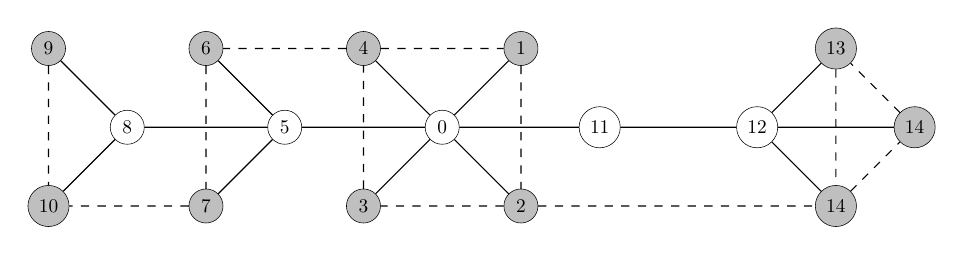
\begin{tikzpicture}
        \wn (n0) at (\coordscl{0}, \coordscl{0}) {0};
        \bn (n1) at (\coordscl{1}, \coordscl{1}) {1};
        \bn (n2) at (\coordscl{1}, \coordscl{-1}) {2};
        \bn (n3) at (\coordscl{-1}, \coordscl{-1}) {3};
        \bn (n4) at (\coordscl{-1}, \coordscl{1}) {4};
        \wn (n5) at (\coordscl{-2}, \coordscl{0}) {5};
        \bn (n6) at (\coordscl{-3}, \coordscl{1}) {6};
        \bn (n7) at (\coordscl{-3}, \coordscl{-1}) {7};
        \wn (n8) at (\coordscl{-4}, \coordscl{0}) {8};
        \bn (n9) at (\coordscl{-5}, \coordscl{1}) {9};
        \bn (n10) at (\coordscl{-5}, \coordscl{-1}) {10};
        \wn (n11) at (\coordscl{2}, \coordscl{0}) {11};
        \wn (n12) at (\coordscl{4}, \coordscl{0}) {12};
        \bn (n13) at (\coordscl{5}, \coordscl{1}) {13};
        \bn (n14) at (\coordscl{5}, \coordscl{-1}) {14};
        \bn (n15) at (\coordscl{6}, \coordscl{0}) {14};

        \draw[dashed]
            (n1) -- (n2)
            (n2) -- (n3)
            (n3) -- (n4)
            (n4) -- (n1)
            (n4) -- (n6)
            (n6) -- (n7)
            (n7) -- (n10)
            (n9) -- (n10)
            (n2) -- (n14)
            (n13) -- (n14)
            (n14) -- (n15)
            (n15) -- (n13)
            ;

        \draw
            (n0) -- (n1)
            (n0) -- (n2)
            (n0) -- (n3)
            (n0) -- (n4)
            (n0) -- (n5)
            (n5) -- (n6)
            (n5) -- (n7)
            (n5) -- (n8)
            (n8) -- (n9)
            (n8) -- (n10)
            (n0) -- (n1)
            (n0) -- (n2)
            (n0) -- (n11)
            (n11) -- (n12)
            (n12) -- (n13)
            (n12) -- (n14)
            (n12) -- (n15)
            ;
    \end{tikzpicture}
        
    \caption{Minimal connecting}
    \label{fig:bmlrp-connect}
\end{figure}
